\documentclass[11pt]{article}
\usepackage[utf8]{inputenc} % Para caracteres en espa�ol
\usepackage{amsmath,amsthm,amsfonts,amssymb,amscd}
\usepackage{multirow,booktabs}
\usepackage[table]{xcolor}
\usepackage{fullpage}
\usepackage{lastpage}
\usepackage{enumitem}

\usepackage{tikz}
\newcommand{\stencilpt}[4][]{\node[circle,draw,inner sep=0.3em,minimum size=2cm,#1] at (#2) (#3) {#4}}
\newcommand{\stencilpta}[4][]{\node[square,draw,inner sep=0.3em,minimum size=2cm,#1] at (#2) (#3) {#4}}



\usepackage{multicol}
\usepackage{fancyhdr}
\usepackage{mathrsfs}
\usepackage{pdfpages}
\usepackage{wrapfig}
\usepackage{setspace}
\usepackage{esvect}
\usepackage{calc}
\usepackage{multicol}
\usepackage{cancel}
\usepackage{graphicx}
\graphicspath{ {pictures/} }
\usepackage[retainorgcmds]{IEEEtrantools}
\usepackage[margin=3cm]{geometry}
\usepackage{amsmath}
\newlength{\tabcont}
\setlength{\parindent}{0.0in}
\setlength{\parskip}{0.05in}
\usepackage{empheq}
\usepackage{framed}
\usepackage[most]{tcolorbox}
\usepackage{xcolor}
\colorlet{shadecolor}{orange!15}
\parindent 0in
\parskip 12pt
\geometry{margin=1in, headsep=0.25in}
\theoremstyle{definition}
\newtheorem{defn}{Definition}
\newtheorem{reg}{Rule}
\newtheorem{exer}{Exercise}
% Two more packages that make it easy to show MATLAB code
\usepackage[T1]{fontenc}
\usepackage[framed,numbered]{matlab-prettifier}
\lstset{
	style = Matlab-editor,
	basicstyle=\mlttfamily\small,
}
\newtheorem{note}{Note}
\begin{document}  
\setcounter{section}{0}
\thispagestyle{empty}

\begin{center}
{\LARGE \bf Homework 4}\\
{\large AE370 - Spring 2018 \\ Emilio R. Gordon}
\end{center}
\vspace{0mm}
\textbf{Problem: Steady-state fluid problem} \\ \\
Use the finite difference method to solve the following incompressible/inviscid fluid flow problem:\\
%\includegraphics[scale=0.7]{1.png}\\
\noindent\makebox[\textwidth]{\includegraphics[scale=0.8]{1.png}}
The flow problem can be described by the following GDE:

\begin{equation*}
\begin{aligned}
\frac{\partial^2 \Phi}{\partial x^2}+\frac{\partial^2 \Phi}{\partial y^2} = 0
\end{aligned}
\end{equation*}

where the streamline function $\Phi$ is related to the x and y components of the velocity vector through:

\begin{equation*}
\begin{aligned}
V_x = \frac{\partial \Phi}{\partial y} \qquad V_y = -\frac{\partial \Phi}{\partial x}
\end{aligned}
\end{equation*}
The boundary conditions are:

\begin{equation*}
\begin{aligned}
\Phi &= V \, y &\qquad \text{along AF}\\
\Phi &=2VH &\qquad \text{along FE}\\
\Phi &=2V(y-H) &\qquad \text{along DE}\\
\Phi &=0 &\qquad \text{along ABCD}\\
\end{aligned}
\end{equation*}
\newpage
Use a second-order central diffrence scheme to solve the problem using N, grid spacings to discretize L (i.e. $\Delta x = L/N_x$) and $N_y$ grid spacings to discretize H (i.e., $\Delta y = H/N_y$).
\begin{enumerate}[label=(\alph*)]
\item Derive the discretized form of the PDE
\item Choose a numbering of the grid points (Describe it thoroughly in your report!) and put together the matrix equation.
\item Implement the boundary conditions.
\item Write a Matlab code that solves this problem. As output you should create the following three plots:
\begin{enumerate}
\item A contour plot for the streamline function (using the command \texttt{CONTOUR})
\item A vector plot for the velocity field (using the central difference approximation for the first derivatives of the streamline function and the command \texttt{QUIVER})
\item A x-y plot of the pressure distribution along the edge boundary condition, where the pressure is obtained by $P = \rho (V_x^2 + V_y^2)$ where $\rho$ is the fluid density.
\end{enumerate}
\item Solve the problem for L=1 [m], H = 0.2 [m], V = 1 [m/s] and $\rho=1 [kg/m^3]$. Perform a convergence study to determine the appropriate values of $N_x$ and $N_y$. Comment on your solution and especially on the computed solution in the vicinity of the corner.
\end{enumerate}

\vfill
{\Large \textbf{Solution:} }
\newpage
\textbf{(a) Derive the discretized form of the PDE}

Before beginning the problem, it is important to classify the PDE's character according to the directions along which information can travel. From class, we learned it is possible to determine a PDE's direction by...
\begin{shaded}
\textbf{Determining PDE Directions}
\begin{equation*}
\begin{aligned}
a \, \frac{\partial^2 T}{\partial x^2} + b \, \frac{\partial^2 T}{\partial x \, \partial y} + c \, \frac{\partial^2 T}{\partial y^2} + d \, \frac{\partial T}{\partial x} + e \, \frac{\partial T}{\partial y} + g \, T + h = 0
\end{aligned}
\end{equation*}

Such that the slope $(dx/dy)$ is controlled by the sign of $(b^2 - 4ac)$. In other words, If...
\begin{equation*}
\begin{aligned}
(b^2 - 4ac) < 0 &\rightarrow \text{the slope is imaginary (all directions)} \\
&\rightarrow \textbf{Elliptic PDE} \\ \\
(b^2 - 4ac) = 0 &\rightarrow \text{There is only one slope (information uniformly in one direction)} \\
&\rightarrow \textbf{Parabolic PDE} \\ \\
(b^2 - 4ac) > 0 &\rightarrow \text{There are two slopes (information in two paths)} \\
&\rightarrow \textbf{Hyperbolic PDE} \\ \\
\end{aligned}
\end{equation*}
\end{shaded}

The general differential equation given $\frac{\partial^2 \Phi}{\partial x^2}+\frac{\partial^2 \Phi}{\partial y^2} = 0$ classifies as an elliptical PDE meaning information travels in all directions.
\\ \\
In part b, a structured grid will be created. For a structured grid, using the second-order central difference approach for x-derivatives and indexing i values for a given y-location (j), we have
\begin{equation*}
\begin{aligned}
\Bigg(\frac{\partial^2 \Phi}{\partial x^2}\Bigg)_{i,j} = \frac{\Phi_{i-1,j} - 2 \Phi_{i,j} + \Phi_{i+1,j}}{\Delta x^2} + O(\Delta x^2)
\end{aligned}
\end{equation*}

For a structured grid, using the second-order central difference approach for y-derivatives and indexing j values for a given x-location (i), we have

\begin{equation*}
\begin{aligned}
\Bigg(\frac{\partial^2 \Phi}{\partial y^2}\Bigg)_{i,j} = \frac{\Phi_{i,j-1} - 2 \Phi_{i,j} + \Phi_{i,j+1}}{\Delta y^2} + O(\Delta y^2)
\end{aligned}
\end{equation*}

Combining these two expressions into our PDE, we get the discretized form of the PDE.
\begin{framed}
\begin{equation*}
\begin{aligned}
\frac{\Phi_{i,j-1} - 2 \Phi_{i,j} + \Phi_{i,j+1}}{\Delta y^2} + \frac{\Phi_{i-1,j} - 2 \Phi_{i,j} + \Phi_{i+1,j}}{\Delta x^2} = 0
\end{aligned}
\end{equation*}
\end{framed}

Expanding

\begin{equation*}
\begin{aligned}
\frac{\Phi_{i,j-1}}{\Delta y^2} - \frac{2 \Phi_{i,j}}{\Delta y^2} + \frac{\Phi_{i,j+1}}{\Delta y^2} + \frac{\Phi_{i-1,j}}{\Delta x^2} - \frac{2 \Phi_{i,j}}{\Delta x^2} + \frac{\Phi_{i+1,j}}{\Delta x^2} = 0
\end{aligned}
\end{equation*}

Simplifying

\begin{equation*}
\begin{aligned}
2 \, \Phi_{i,j} \, (\Delta x^2 + \Delta y^2) = \Delta x^2 \, (\Phi_{i,j-1} + \Phi_{i,j+1}) + \Delta y^2 \, (\Phi_{i-1,j} + \Phi_{i+1,j})
\end{aligned}
\end{equation*}
\\ \\
Divide by $\Delta y^2$ and define $\eta = \frac{\Delta x}{ \Delta y}$ such that

\begin{equation*}
\begin{aligned}
2 \, \Phi_{i,j} \, (1 + \eta^2) = \eta^2 \, (\Phi_{i,j-1} + \Phi_{i,j+1}) + (\Phi_{i-1,j} + \Phi_{i+1,j})
\end{aligned}
\end{equation*}
\\ \\
Our final discretized GDE therefore is...

\begin{framed}
\begin{equation*}
\begin{aligned}
 0 =\eta^2 \, \Phi_{i,j-1} + \eta^2 \, \Phi_{i,j+1} -2 \, \Phi_{i,j} \, (1 + \eta^2) + \Phi_{i-1,j} + \Phi_{i+1,j}
\end{aligned}
\end{equation*}
Where
\begin{equation*}
\begin{aligned}
\eta = \frac{\Delta x}{\Delta y}
\end{aligned}
\end{equation*}
\end{framed}

\newpage
\textbf{(b) Choose a numbering of the grid points and put together the matrix equation.}

From the code provided, it is easy to extrapolate the Global Equation Number (GEN) by the problem. The shape of the duct adds some complexities to calculating the GEN  however, it is simple enough to look at in sections. NOTE: The figure in the code provided differs from the problem statement figure. The figure provided in the code was used in this analysis.
\\
\begin{figure}[h!]
\begin{lstlisting}
%     B                        E                       G
%     --------------------------------------------------
%     |                                                |
%     |                                                |
%     |                                                |
%     |                                                |
%     |                                                |
%     |                         D                      |F
%     |                         ------------------------
%     |                         |
%     |                         |
%     |                         |
%     |                         |
%     |                         |
%     |                         |
%     ---------------------------
%    A                          C
%
% Dimensions:    AC = DF = BE = EG = L
%                CD = FG = DE = AB/2 = H
% The domain is discretized with Nx grid spacings along AC and DF
% and NY grid spacings along CD and FG.
% Index convention:
%     Local indices (i,j)         Global index (q)
%   A      (1,1)                         qA=1
%   B      (1,2*Ny+1)                    qB=2*Ny+1
%   C      (Nx+1,1)                      qC=Nx*(2*Ny+1)+1
%   D      (Nx+1,Ny+1)                   qD=qC+Ny
%   E      (Nx+1,2*Ny+1)                 qE=qD+Ny
%   F      (2*Nx+1,Ny+1)                 qF=qE+(Nx-1)*(Ny+1)+1
%   G      (2*Nx+1,2*Ny+1)               qG=qF+Ny
\end{lstlisting}
\caption{Problem Diagram and Index Convention}
\end{figure}
\\
The Duct can be divided into two sections: ABEDC and DEGF. The only notable difference is the lack of a bottom half on the second section. In addition, we already know the GEN of the corners given Nx and Ny. The order at which the GEN are defined will be as follows:
\begin{enumerate}[label=(\arabic*)]
\item Start at the A corner, GEN = 1
\item Move upward till we reach point B, (i=1, j=2Ny+1)
\item Shift to the bottom of the next column and repeat.
\end{enumerate}

In class, we were given the equation $GEN = i + (j-1)n$, where $i$ and $j$ are the indices and $n$ is the column number. Building on this, a GEN for section ABEDC can be made understanding that the section ends when $i = Nx + 1$. As a result, it can be said that so long as $i \leq Nx + 1$ then $q = (i-1) \, (2 Ny+1)+j$ essentially applying a GEN as described above.
\\ \\
The above GEN equation only applies when $i \leq Nx + 1$, section ABEDC. The second section, section DEGF, has the physical constraint of not existing for any points below $Ny+1$. Keeping with the GEN ordering system defined above for the second section, it can be said that so long as $j \geq Ny+1$ then $q = (Nx + 1)\,(2Ny+1)+(i-Nx-2)(Ny+1)+j-Ny$. 
\\ \\
Any other possible value for the global equation number falls outside of the shape and is set to 0.
\\ \\
To summarize, calculating the Global Equation Number is done by the following function. 
\\
\begin{figure}[h!]
\begin{lstlisting}
function q=compute_q(i,j,Nx,Ny)
q = 0;
    if(i <= Nx +1)
        q = (i-1)*(2*Ny+1)+j; 
    elseif(j >= Ny + 1)
        q = (Nx + 1)*(2*Ny+1)+(i-Nx-2)*(Ny+1)+j-Ny;
    end
end
\end{lstlisting}
\caption{Subroutine to Compute the Global Equation Number Corresponding to Grid}
\end{figure}
\\
With this model in place, we can now start forming the linear system. Keeping with the form of $Au = b$ the following code was used to establish an A matrix, the matrix of our knowns. 
\\ \\
From part 1, we arrived at a formula for the discretized PDE of
\begin{equation*}
\begin{aligned}
 0 =\eta^2 \, \Phi_{i,j-1} + \eta^2 \, \Phi_{i,j+1} -2 \, \Phi_{i,j} \, (1 + \eta^2) + \Phi_{i-1,j} + \Phi_{i+1,j}
\end{aligned}
\end{equation*}
Where
\begin{equation*}
\begin{aligned}
\eta = \frac{\Delta x}{\Delta y}
\end{aligned}
\end{equation*}
\newpage
From this, a five-point computational stencil for each node (i,j) is constructed.
\\
\begin{figure}[h!]
\begin{center}
\begin{tabular}{ c c c}
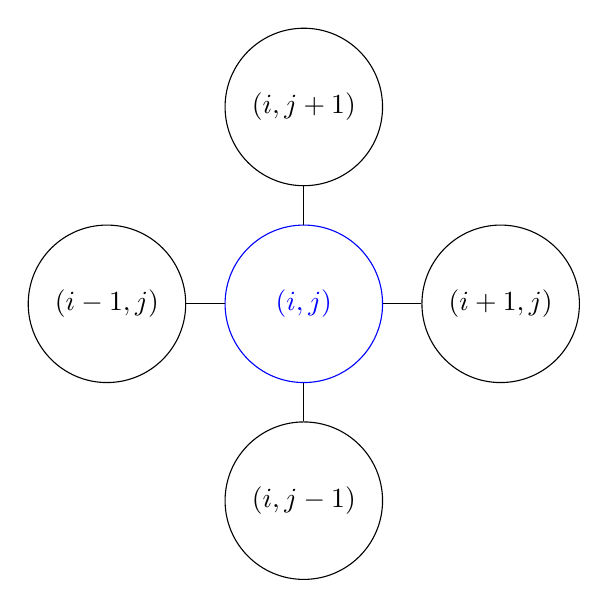
\begin{tikzpicture}
  \stencilpt{-2.5,0}{i-1}{$(i-1,j)$};
  \stencilpt[blue]{ 0,0}{i}  {$(i,j)$};
  \stencilpt{ 2.5,0}{i+1}{$(i+1,j)$};
  \stencilpt{0,-2.5}{j-1}{$(i,j-1)$};
  \stencilpt{0, 2.5}{j+1}{$(i,j+1)$};
  \draw
        (j-1) -- (i)
        (i)   -- (j+1)
        (i-1) -- (i)
        (i)   -- (i+1);
\end{tikzpicture} &\quad $\rightarrow$ \quad \vspace{10mm} & \begin{tikzpicture}
  \stencilpt{-2.5,0}{i-1}{$1$};
  \stencilpt[blue]{ 0,0}{i}  {$-2 \, (1 + \eta^2)$};
  \stencilpt{ 2.5,0}{i+1}{$1$};
  \stencilpt{0,-2.5}{j-1}{$\eta^2$};
  \stencilpt{0, 2.5}{j+1}{$\eta^2$};
  \draw
        (j-1) -- (i)
        (i)   -- (j+1)
        (i-1) -- (i)
        (i)   -- (i+1);
\end{tikzpicture}
\end{tabular}
\end{center}
\caption{Five-Point Computational Stencil}
\end{figure}
\\
It is easier to start forming a linear system by filling in the interior. The code in Figure \ref{FormA} does this by
\begin{enumerate}
\item First establishing a zero "sparse" matrix with dimensions $m \times n$ where m and n are both the number of nodes in the system.
\item Step 1 is set as a placeholder along the diagonal for all degrees of freedom. These are later overwritten by the interior grid points for the appropriate cells.
\item We are only focusing on the interior. Therefore, for the ABEDC section, we parse over
\begin{itemize}
\item $i = 2:Nx$ 
\begin{itemize}
\item 2: Starting at the second column
\item $Nx$: Ending right before the boundary condition $Nx+1$
\end{itemize}
\item $j = 2:2 \, Ny$ 
\begin{itemize}
\item 2: Starting at the second row
\item $2 \, Ny$: Ending right before the boundary condition $2 \,Ny+1$
\end{itemize}
\end{itemize}
\item Again, we are only focusing on the interior. Therefore, for the DEGF section, we parse over
\begin{itemize}
\item $i = Nx+1:2 \, Nx$ 
\item $j = Ny+2:2 \, Ny$ 
\end{itemize}
\end{enumerate}
\newpage
\begin{figure}[h!]
\begin{lstlisting}
% Set up matrix (Amat) and vector (bvec) dimensions
Amat=sparse(Numeq,Numeq);
bvec=zeros(Numeq,1);
%
% Build linear system
for i=1:Numeq;       % place 1 along diagonal for all DOF then overwrite the interior grid points
    Amat(i,i)=1;
end
for i=2:Nx % loop over interior grid points - left half of domain
    for j=2:2*Ny
        qij=compute_q(i,j,Nx,Ny); % compute equation number q for(i,j) grid point 
        Amat(qij,qij)=-2*(1+eta^2);%Grid Point
        q=compute_q(i-1,j,Nx,Ny); %Grid Point to the left
        Amat(qij,q)= 1;
        q=compute_q(i+1,j,Nx,Ny); %Grid Point to the right
        Amat(qij,q)= 1;
        q=compute_q(i,j-1,Nx,Ny); % Grid point below
        Amat(qij,q)= eta^2;
        q=compute_q(i,j+1,Nx,Ny); %Grid Point above
        Amat(qij,q)= eta^2;
    end
end
for i=Nx+1:2*Nx % loop over interior grid points - right half of domain
    for j=Ny+2:2*Ny
        qij=compute_q(i,j,Nx,Ny);
        Amat(qij,qij)= -2*(1+eta^2);
        q=compute_q(i-1,j,Nx,Ny);
        Amat(qij,q)= 1;
        q=compute_q(i+1,j,Nx,Ny);
        Amat(qij,q)= 1;
        q=compute_q(i,j-1,Nx,Ny);
        Amat(qij,q)= eta^2;
        q=compute_q(i,j+1,Nx,Ny);
        Amat(qij,q)= eta^2;
    end
end
\end{lstlisting}
\caption{Building the A Matrix for the Linear System}
\label{FormA}
\end{figure}
\newpage
\textbf{Implement the boundary conditions.}

Implementing the boundary conditions posses a set of challenges. We will tackle this by focusing on them individually. 

We start with
\begin{equation*}
\begin{aligned}
\Phi &=2VH &\qquad \text{along FE}\\
\end{aligned}
\end{equation*}

To implement this, it is required to define the nodes it is applied to. Simply put, a boundary condition along FE means that for the condition applies for $\Phi(x,2H)$. In terms our indices
\begin{itemize}
\item $i = 2:2 \, Nx$ 
\begin{itemize}
\item Starting at the second column
\item Boundary condition applies till the second to last column
\end{itemize}
\item $j = 2 \, Ny+1$ 
\begin{itemize}
\item Constant
\item Fixed at the top edge of the boundary.
\end{itemize}
\end{itemize}
\begin{figure}[h!]
\begin{lstlisting}
for i=2:2*Nx
    j=2*Ny+1;
    q=compute_q(i,j,Nx,Ny);
    bvec(q)= 2*V*H; %Boundary Condition
end
\end{lstlisting}
\caption{Implementing Boundary Conditions Over the Top Edge}
\label{}
\end{figure}
\newpage
Next we implement
\begin{equation*}
\begin{aligned}
\Phi &=2V(y-H) &\qquad \text{along DE}\\
\end{aligned}
\end{equation*}

To implement this, it is required to define the nodes it is applied to. Simply put, a boundary condition along DE means that for the condition applies for $\Phi(2L,y)$. In terms our indices
\begin{itemize}
\item $i = 2\,Nx+1$ 
\begin{itemize}
\item Constant
\item Fixed at the right edge of the boundary.
\end{itemize}
\item $j = Ny+1:2 \, Ny + 1$ 
\begin{itemize}
\item Starting from the bottom of section DEGF
\item Ending at the top of section DEGF
\end{itemize}
\end{itemize}
\begin{figure}[h!]
\begin{lstlisting}
for j=Ny+1:2*Ny+1
    i=2*Nx+1;
    q=compute_q(i,j,Nx,Ny);
    y = (j-1)*dy;
    bvec(q)= 2*V*(y-H); %Boundary Condition
end
\end{lstlisting}
\caption{Implementing Boundary Conditions Over the Right Edge}
\label{}
\end{figure}
%\newpage
Finally, the last non-zero boundary condition is
\begin{equation*}
\begin{aligned}
\Phi &=V \, y &\qquad \text{along AF}\\
\end{aligned}
\end{equation*}
To implement this, it is required to define the nodes it is applied to. Simply put, a boundary condition along AF, means that for the condition applies for $\Phi(1,y)$. In terms our indices
\begin{itemize}
\item $j = 1:2 \, Ny + 1$ 
\begin{itemize}
\item Starting from the bottom of line AF
\item Ending at the top of section AF
\end{itemize}
\end{itemize}
\begin{figure}[h!]
\begin{lstlisting}
for j=1:2*Ny+1
    bvec(j)= V*(j-1)*dy;
end
\end{lstlisting}
\caption{Implementing Boundary Conditions Over the Left Edge}
\label{}
\end{figure}
\newpage
\begin{figure}[h!]
\begin{lstlisting}
%
% Build right-hand-side vector (imposed Psi BC)
for j=1:2*Ny+1 % loop over the left edge:
    bvec(j)= V*(j-1)*dy;
end
for i=2:2*Nx % loop over top edge:
    j=2*Ny+1;
    q=compute_q(i,j,Nx,Ny);
    bvec(q)= 2*V*H;
end
for j=Ny+1:2*Ny+1 % loop over right edge:
    i=2*Nx+1;
    q=compute_q(i,j,Nx,Ny);
    y = (j-1)*dy;
    bvec(q)= 2*V*(y-H);
end
% Remainder of boundary has Psi=0
\end{lstlisting}
\caption{Building the B Matrix for the Linear System}
\label{}
\end{figure}

\newpage
\textbf{Write a Matlab code that solves this problem and output the following three plots:}

The complete code can be found on the final pages of this report.

A contour plot for the streamline function is shown in Figure \ref{fig:ContourStream}. Here, the contours represent the computed function, $\Phi (x,y)$. Note that the sharper gradient on the right side of the domain. This is an indication of acceleration of the fluid flow which is expected for incompressible flow.
\\
\begin{figure}[h!]
\label{fig:ContourStream}
\begin{center}
\includegraphics[scale=0.6]{contourStream.pdf}
\end{center}

\caption{Contour Plot of the Streamline Function $\Phi (x,y)$}
\end{figure}
\newpage
A vector plot for the velocity field using the central difference approximation for the first derivatives of the streamline function is shown in Figure \ref{fig:VelocityDistribution}. Differentiating the streamline function field, $\Phi (x,y)$ is done by using the central difference scheme for the interior nodes and then the forward finite difference scheme for the boundary nodes. The results show, as suggested from before, an acceleration of the flow past the step. In addition, the velocity field also shows high velocity at the corner of the step.
\\
\begin{figure}[h!]
\label{fig:VelocityDistribution}
\begin{center}
\includegraphics[scale=0.6]{vfield.pdf}
\end{center}
\caption{Velocity Vector Field for the Streamline Function $\Phi (x,y)$}
\end{figure}
\newpage
The dynamic pressure field along the edge boundary condition is obtained by $P = \frac{1}{2} \,\rho \, (V_x^2 + V_y^2)$ where $\rho$ is the fluid density and is shown in Figure \ref{fig:PressureContour}. It becomes clear that there is high pressure at the corner which is expected do to the higher velocity. Increasing Ny to create a finer discretization (noting that Nx is always 2Ny).
\\
\begin{figure}[h!]
\label{fig:PressureContour}
\begin{center}
\includegraphics[scale=0.7]{contourPressure.pdf}
\end{center}
\caption{Pressure Field for Various Values of Ny. Note Nx = 2 Ny}
\end{figure}
\newpage
This becomes even more clear when zooming in on the corner as shown in Figure \ref{fig:PressureContourZoomed}
\\
\begin{figure}[h!]
\label{fig:PressureContourZoomed}
\begin{center}
\includegraphics[scale=0.7]{contourPressureZoomed.pdf}
\end{center}
\caption{Pressure Field Zoomed Corner View}
\end{figure}
\\
The extremely volatile pressure gradient seen at the corner attributes to convergence issues at the corner.
\newpage
\textbf{Solve the problem for L=1 [m], H = 0.2 [m], V = 1 [m/s] and $\rho=1 [kg/m^3]$. Perform a convergence study to determine the appropriate values of $N_x$ and $N_y$. Comment on your solution and especially on the computed solution in the vicinity of the corner.}
\\ \\
Finally, the evolution of the pressure along the vertical segment (side CD) is shown in the figures below for four different discretizations.
\\
\begin{figure}[h!]
\label{fig:PressureContourZoomed}
\begin{center}
\includegraphics[scale=0.6]{PressurePlots.pdf}
\end{center}
\caption{Pressure Values along CD}
\end{figure}
\newpage
From these plots, it can be shown how the solution is convergent along the vertical step, diverging only when approaching the vicinity of the corner. This is a result of the extremely high gradient present at the corner. Figure 14 below examines more closely how the divergence is more apparent in the vicinity of the corner. 
\\
\begin{figure}[h!]
\label{fig:PressureContourZoomed}
\begin{center}
\includegraphics[scale=0.6]{PressurePlotsZoomed.pdf}
\end{center}
\caption{Zoomed Pressure Values along CD }
\end{figure}
\newpage
Another way to solve for convergence of the entire system is to examine information regarding the exit velocity. It is understood that at the exit plane, the velocity at the top will be 2 m/s and at the lower end, 1 m/s. This means that the average output velocity is 1.5m/s. Using this information, we can compute the velocity for different subdivisions of Ny (keeping Nx = 2 Ny), compute the mean exit plane velocity and calculated the relative error, knowing that the exact average velocity must be 1.5. 
\\
\begin{figure}[h!]
\label{fig:PressureContourZoomed}
\begin{center}
\includegraphics[scale=0.6]{vError.pdf}
\end{center}
\caption{Relative Velocity Error at Exit Plane}
\end{figure}
\\
From the relative velocity error study, an estimate for a good Nx and Ny values are:

\begin{equation*}
\begin{aligned}
(N_x, N_y) = (80,40)
\end{aligned}
\end{equation*}

These values are also supported by the pressure study from Figure 12 and Figure 13. Though increasing the Ny and Nx values will produced better results, it can be shown that the estimated results from $(N_x, N_y) = (80,40)$ is sufficient enough to provide accurate data at reasonable computation speeds. 

\newpage
Complete Code
\begin{lstlisting}
% Program StepFlow
% Finite difference code to solve the problem of an inviscid,
% incompressible flow going over a step.
% 
%
%     B                        E                       G
%     --------------------------------------------------
%     |                                                |
%     |                                                |
%     |                                                |
%     |                                                |
%     |                                                |
%     |                         D                      |F
%     |                         ------------------------
%     |                         |
%     |                         |
%     |                         |
%     |                         |
%     |                         |
%     |                         |
%     ---------------------------
%    A                          C
%
% Dimensions:    AC = DF = BE = EG = L
%                CD = FG = DE = AB/2 = H
% The domain is discretized with Nx grid spacings along AC and DF
% and NY grid spacings along CD and FG.
% Index convention:
%     Local indices (i,j)         Global index (q)
%   A      (1,1)                         qA=1
%   B      (1,2*Ny+1)                    qB=2*Ny+1
%   C      (Nx+1,1)                      qC=Nx*(2*Ny+1)+1
%   D      (Nx+1,Ny+1)                   qD=qC+Ny
%   E      (Nx+1,2*Ny+1)                 qE=qD+Ny
%   F      (2*Nx+1,Ny+1)                 qF=qE+(Nx-1)*(Ny+1)+1
%   G      (2*Nx+1,2*Ny+1)               qG=qF+Ny
%
function StepFlow
close all; clear all; clc;
% Key parameters
L = 1; %x-dimension of domain (m)
H = 0.2; %y-direction of step (m)

Ny1= 20; %input(' Enter number of grid spacings in y (Ny) ')
Nx1= 2*Ny1; %input(' Enter number of grid spacings in x (Nx) ')
Ny2 = 40;
Nx2 = 2*Ny2;
Ny3 = 80;
Nx3 = 2*Ny3;
Ny4 = 160;
Nx4 = 2*Ny4;

dx1=L/Nx1;  % grid spacing in x direction
dy1=H/Ny1;  % grid spacing in y direction
dx2=L/Nx2;  
dy2=H/Ny2;  
dx3=L/Nx3;  
dy3=H/Ny3;  
dx4=L/Nx4;  
dy4=H/Ny4;  

V=1;    % imposed inflow velocity (in m/s) (the outflow velocity = 2V)
rho=1;  % fluid density (in kg/m^3) (to compute the dynamic pressure)

Psimat1 = computeStream(Nx1, Ny1,L,H,V,dx1,dy1);
Psimat2 = computeStream(Nx2, Ny2,L,H,V,dx2,dy2);
Psimat3 = computeStream(Nx3, Ny3,L,H,V,dx3,dy3);
Psimat4 = computeStream(Nx4, Ny4,L,H,V,dx4,dy4);

plotContour(Psimat4,Nx4,Ny4,L,H)

figure(2)
plotVectorField(Psimat1,Nx1,Ny1,L,H,V,dx1,dy1)

figure(3)
subplot(2, 2,1);
plotContourPressures(Psimat1,Nx1,Ny1,L,H,V,dx1,dy1,rho)
subplot(2, 2,2);
plotContourPressures(Psimat2,Nx2,Ny2,L,H,V,dx2,dy2,rho)
subplot(2, 2,3);
plotContourPressures(Psimat3,Nx3,Ny3,L,H,V,dx3,dy3,rho)
subplot(2, 2,4);
plotContourPressures(Psimat4,Nx4,Ny4,L,H,V,dx4,dy4,rho)

figure(5)
subplot(2, 2,1);
plotContourPressuresZoomed(Psimat1,Nx1,Ny1,L,H,V,dx1,dy1,rho)
subplot(2, 2,2);
plotContourPressuresZoomed(Psimat2,Nx2,Ny2,L,H,V,dx2,dy2,rho)
subplot(2, 2,3);
plotContourPressuresZoomed(Psimat3,Nx3,Ny3,L,H,V,dx3,dy3,rho)
subplot(2, 2,4);
plotContourPressuresZoomed(Psimat4,Nx4,Ny4,L,H,V,dx4,dy4,rho)

figure(4)
plotPressures(Psimat1,Psimat2, Psimat3, Psimat4,Nx1,Ny1,Nx2,Ny2,Nx3,Ny3,Nx4,Ny4,H,V,dx1,dy1,dx2,dy2,dx3,dy3,dx4,dy4,rho)

end

function [Psimat] = computeStream(Nx, Ny, L, H,V,dx,dy)
eta=dx/dy;  % grid spacing ratio
rho=1;  % fluid density (in kg/m^3) (to compute the dynamic pressure)

% Compute global equation number of corners (see schematic above)
qA=1;
qB=2*Ny+1;        % N
qC=Nx*(2*Ny+1)+1; % Nx*(qB)+1
qD=qC+Ny;
qE=qD+Ny;
qF=qE+(Nx-1)*(Ny+1)+1;
qG=qF+Ny;
Numeq=qG;     % number of equations
%
% Set up matrix (Amat) and vector (bvec) dimensions
Amat=sparse(Numeq,Numeq);
bvec=zeros(Numeq,1);
% Build linear system
for i=1:Numeq;       % place 1 along diagonal for all DOF then overwrite the interior grid points
    Amat(i,i)=1;
end
for i=2:Nx % loop over interior grid points - left half of domain
    for j=2:2*Ny
        qij=compute_q(i,j,Nx,Ny); % compute equation number q for(i,j) grid point 
        Amat(qij,qij)=-2*(1+eta^2);%Grid Point
        q=compute_q(i-1,j,Nx,Ny); %Grid Point to the left
        Amat(qij,q)= 1;
        q=compute_q(i+1,j,Nx,Ny); %Grid Point to the right
        Amat(qij,q)= 1;
        q=compute_q(i,j-1,Nx,Ny); % Grid point below
        Amat(qij,q)= eta^2;
        q=compute_q(i,j+1,Nx,Ny); %Grid Point above
        Amat(qij,q)= eta^2;
    end
end
for i=Nx+1:2*Nx % loop over interior grid points - right half of domain
    for j=Ny+2:2*Ny
        qij=compute_q(i,j,Nx,Ny);
        Amat(qij,qij)= -2*(1+eta^2);
        q=compute_q(i-1,j,Nx,Ny);
        Amat(qij,q)= 1;
        q=compute_q(i+1,j,Nx,Ny);
        Amat(qij,q)= 1;
        q=compute_q(i,j-1,Nx,Ny);
        Amat(qij,q)= eta^2;
        q=compute_q(i,j+1,Nx,Ny);
        Amat(qij,q)= eta^2;
    end
end


%
% Build right-hand-side vector (imposed Psi BC)
for j=1:2*Ny+1 % loop over the left edge:
    bvec(j)= V*(j-1)*dy;
end
for i=2:2*Nx % loop over top edge:
    j=2*Ny+1;
    q=compute_q(i,j,Nx,Ny);
    bvec(q)= 2*V*H;
end
for j=Ny+1:2*Ny+1 % loop over right edge:
    i=2*Nx+1;
    q=compute_q(i,j,Nx,Ny);
    y = (j-1)*dy;
    bvec(q)= 2*V*(y-H);
end
% Remainder of boundary has Psi=0
%
% Solve linear system
Psivec=Amat\bvec;
% Build Psi array for visualization (fill lower right with zero
Psimat=zeros(2*Nx+1,2*Ny+1);
for i=1:2*Nx+1     % loop over all points in domain
    for j=1:2*Ny+1
        q=compute_q(i,j,Nx,Ny);
        if q == 0    % if inside step region, assign Phi=0
            Psimat(i,j)=0;
        else  % if inside computational domain, extra Phi value from solution vector
            Psimat(i,j)=Psivec(q);
        end
    end
end
end

function q=compute_q(i,j,Nx,Ny)
% Subroutine to compute the global equation number corresponding to grid
% point (i,j)
q = 0;
if(i <= Nx +1)
    q = (i-1)*(2*Ny+1)+j;
elseif(j >= Ny + 1)
    q = (Nx + 1)*(2*Ny+1)+(i-Nx-2)*(Ny+1)+j-Ny;
end
end

function plotContour(Psimat,Nx,Ny,L,H)

xvec=linspace(0,2*L,2*Nx+1);    % vector with 2*Nx+1 values of x
yvec=linspace(0,2*H,2*Ny+1);    % vector with 2*Ny+1 values of y
contourf(xvec,yvec,Psimat',15)  % create filled contour plots of phi field
colormap(jet);
xlabel('x (m)');
ylabel('y (m)');
title('Contour plot of function Phi');
set(gcf,'paperorientation','landscape');
set(gcf,'paperunits','normalized');
set(gcf,'paperposition',[0 0 1 1]);
print(gcf,'-dpdf','contourStream.pdf');
end

function [vx,vy] = Velocity(Psimat,Nx,Ny,V,dx,dy)
vx=zeros(2*Nx+1,2*Ny+1);    % x-component of velocity at each grid point
vy=zeros(2*Nx+1,2*Ny+1);    % y-component of velocity at each grid point

for j=1:2*Ny+1     % left edge
    vx(1,j)=V;
    vy(1,j)=0;
end
for j=Ny+1:2*Ny+1   % right edge
    vx(2*Nx+1,j)=2*V;
    vy(2*Nx+1,j)=0;
end
for i=2:2*Nx       % top edge (backward difference)
    vx(i,2*Ny+1)=(Psimat(i,2*Ny+1)-Psimat(i,2*Ny))/dy;
    vy(i,2*Ny+1)=0;
end
for i=2*Nx         % bottom edge (forward difference)
    vx(i,1)=(Psimat(i,2)-Psimat(i,1))/dy;
end
for i=2:2*Nx         % interior nodes
    for j=2:2*Ny
        vx(i,j)=(Psimat(i,j+1)-Psimat(i,j-1))/2/dy;
        vy(i,j)=-(Psimat(i+1,j)-Psimat(i-1,j))/2/dx;
    end
end
end


function plotVectorField(Psimat,Nx,Ny,L,H,V,dx,dy)
% Compute and display velocity vector field

xvec=linspace(0,2*L,2*Nx+1);    % vector with 2*Nx+1 values of x
yvec=linspace(0,2*H,2*Ny+1);

[vx,vy]=Velocity(Psimat,Nx,Ny,V,dx,dy);

[x,y]=meshgrid(xvec,yvec);
quiver(x',y',vx,vy);    % create vector plot
xlabel('x (m)');
ylabel('y (m)');
axis([0 2 0 1])
title(' Velocity vector plot');
set(gcf,'paperorientation','landscape');
set(gcf,'paperunits','normalized');
set(gcf,'paperposition',[0 0 1 1]);
print(gcf,'-dpdf','vfield.pdf');
end


function plotContourPressures(Psimat,Nx,Ny,L,H,V,dx,dy,rho)
[vx,vy] = Velocity(Psimat,Nx,Ny,V,dx,dy);
% Compute and display pressure field
xvec=linspace(0,2*L,2*Nx+1);    % vector with 2*Nx+1 values of x
yvec=linspace(0,2*H,2*Ny+1);

pressure=0.5*rho*(vx.^2+vy.^2);    % pressure array
contourf(xvec,yvec,pressure',30)     % filled contour plot of pressure field
colormap(jet);
colorbar
xlabel('x (m)');
ylabel('y (m)');
title(sprintf('Pressure Field w/ Ny = %d',Ny));
set(gcf,'paperorientation','landscape');
set(gcf,'paperunits','normalized');
set(gcf,'paperposition',[0 0 1 1]);
print(gcf,'-dpdf','contourPressure.pdf');
end

function plotContourPressuresZoomed(Psimat,Nx,Ny,L,H,V,dx,dy,rho)
[vx,vy] = Velocity(Psimat,Nx,Ny,V,dx,dy);
% Compute and display pressure field
xvec=linspace(0,2*L,2*Nx+1);    % vector with 2*Nx+1 values of x
yvec=linspace(0,2*H,2*Ny+1);

for i = 1:length(xvec)
    if xvec(i) == 0.8
        xLow = i
    end
    if xvec(i) == 1.3
        xHigh = i
    end
end
for i = 1:length(yvec)
    if yvec(i) == 0.4
        yLow = i
    end
    if yvec(i) == 0.6
        yHigh = i
    end
end
pressure=0.5*rho*(vx.^2+vy.^2);    % pressure array
contourf(xvec(xLow:xHigh),yvec(yLow:yHigh),pressure(xLow:xHigh,yLow:yHigh)',(Ny/2)+5)     % filled contour plot of pressure field
colormap(jet);
colorbar
xlabel('x (m)');
ylabel('y (m)');
title(sprintf('Pressure Field w/ Ny = %d',Ny));
set(gcf,'paperorientation','landscape');
set(gcf,'paperunits','normalized');
set(gcf,'paperposition',[0 0 1 1]);
print(gcf,'-dpdf','contourPressureZoomed.pdf');
end

function plotPressures(Psimat1,Psimat2, Psimat3, Psimat4,Nx1,Ny1,Nx2,Ny2,Nx3,Ny3,Nx4,Ny4,H,V,dx1,dy1,dx2,dy2,dx3,dy3,dx4,dy4,rho)
[vx1,vy1] = Velocity(Psimat1,Nx1,Ny1,V,dx1,dy1);
[vx2,vy2] = Velocity(Psimat2,Nx2,Ny2,V,dx2,dy2);
[vx3,vy3] = Velocity(Psimat3,Nx3,Ny3,V,dx3,dy3);
[vx4,vy4] = Velocity(Psimat4,Nx4,Ny4,V,dx4,dy4);

pressure1=0.5*rho*(vx1.^2+vy1.^2)
pressure2=0.5*rho*(vx2.^2+vy2.^2);
pressure3=0.5*rho*(vx3.^2+vy3.^2);
pressure4=0.5*rho*(vx4.^2+vy4.^2);

yvalues1=linspace(0,H,Ny1+1);     % vector with Ny+1 values of y along CD
yvalues2=linspace(0,H,Ny2+1);
yvalues3=linspace(0,H,Ny3+1);
yvalues4=linspace(0,H,Ny4+1);

pvalues1(1:Ny1+1)=pressure1(Nx1+1,1:Ny1+1)  % extract pressure values along CD from pressure array
pvalues2(1:Ny2+1)=pressure2(Nx2+1,1:Ny2+1);
pvalues3(1:Ny3+1)=pressure3(Nx3+1,1:Ny3+1);
pvalues4(1:Ny4+1)=pressure4(Nx4+1,1:Ny4+1);

plot(yvalues1,pvalues1,'bo-','linewidth',2)
hold on
plot(yvalues2,pvalues2,'rs-','linewidth',2)
hold on
plot(yvalues3,pvalues3,'g--','linewidth',2)
hold on
plot(yvalues4,pvalues4,'m+-','linewidth',2)
xlabel('y (m)');
ylabel('pressure (Pa)');
%axis([0.19 0.2 0 6])
title(' Pressure distribution along side CD');
legend(sprintf('N_y = %d',Ny1),sprintf('N_y = %d',Ny2),sprintf('N_y = %d',Ny3),sprintf('N_y = %d',Ny4),'Location','northwest')
set(gcf,'paperorientation','landscape');
set(gcf,'paperunits','normalized');
set(gcf,'paperposition',[0 0 1 1]);
print(gcf,'-dpdf','PressurePlots.pdf');
end
\end{lstlisting}

\end{document}